This is the data that 
I am adding to the project.

\begin{figure}[h]
  \centering
  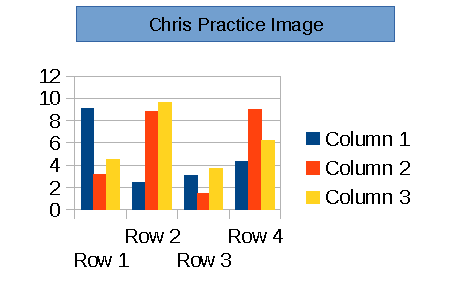
\includegraphics[scale=0.64]{figs/practiceimage}
  \caption{My image for practice. }
  \label{fig:practiceimage}
\end{figure}

This paragraph will show things like
{\em italics} and {\bf bold}.  Also,
I can add comments in two ways.
% Percent starts a comment
50\% of the time you want a slash
in front.  
\MYcomment{If type 
sdsd
dsd
sdsd
ds
dsd
sds}
\MYfigureref{fig:practiceimage} is great!

